\newpage
\section*{CHAPTER 2. THEORETICAL BACKGROUND}
\phantomsection\addcontentsline{toc}{section}{CHAPTER 2. THEORETICAL BACKGROUND}
\setcounter{section}{2}
\setcounter{subsection}{0}
\setcounter{subsubsection}{0}
\setcounter{figure}{0}
\setcounter{table}{0}

Chapter 2 presents the theoretical background required for the design and implementation of the proposed quantized HiFiC GAN accelerator. The chapter first reviews convolutional neural networks (CNNs) and their fundamental layers, since the generator network in learned image compression is dominated by convolution, normalization, activation, residual, and up-sampling operations. It then introduces Generative Adversarial Networks (GANs) and the HiFiC architecture used for learned image compression, followed by the mixed-precision quantization concept that underpins the proposed accelerator. Next, the chapter presents the evaluation metrics for both hardware efficiency and image-compression quality, summarizes the FPGA platform used for hardware acceleration, and introduces High-Level Synthesis (HLS), explaining why HLS is suitable for this thesis and discussing the HLS pragmas used to transform the ResBlock algorithm into an efficient FPGA circuit. Finally, it reviews the software tools used in the design flow.

\subsection{Convolutional Neural Networks}

\subsubsection{Overview of Convolutional Neural Networks}

Convolutional Neural Networks (CNNs) are a major class of deep learning models designed for processing data with spatial structure \cite{ajit2020review}. They are especially effective for two-dimensional visual data such as images, where neighboring pixels usually have strong correlations. Instead of treating every input element independently, CNNs exploit local spatial relationships through convolutional filters. This property makes CNNs suitable for many computer vision tasks, including image classification, object detection, image segmentation, image restoration, and learned image compression.

The operation of a CNN can be interpreted as a hierarchical feature extraction process. In the first layers, the network usually learns simple visual patterns such as edges, corners, color transitions, and local textures. As the data propagates through deeper layers, these low-level patterns are gradually combined into more abstract representations, such as object parts, semantic regions, or compact latent features. In learned image compression systems, this hierarchical representation is important because the encoder network must transform the input image into a compressed latent representation while preserving perceptually meaningful information for the decoder.

A general CNN architecture is shown in Figure~\ref{fig:cnn-overview}. The input image is processed by a sequence of convolutional blocks. Each block commonly contains a convolutional layer, a nonlinear activation function, and sometimes additional operations such as normalization or pooling. For image compression and generative models, the network may also include down-sampling layers in the encoder to reduce spatial resolution and produce compact latent features.

\begin{figure}[htbp]
    \centering
    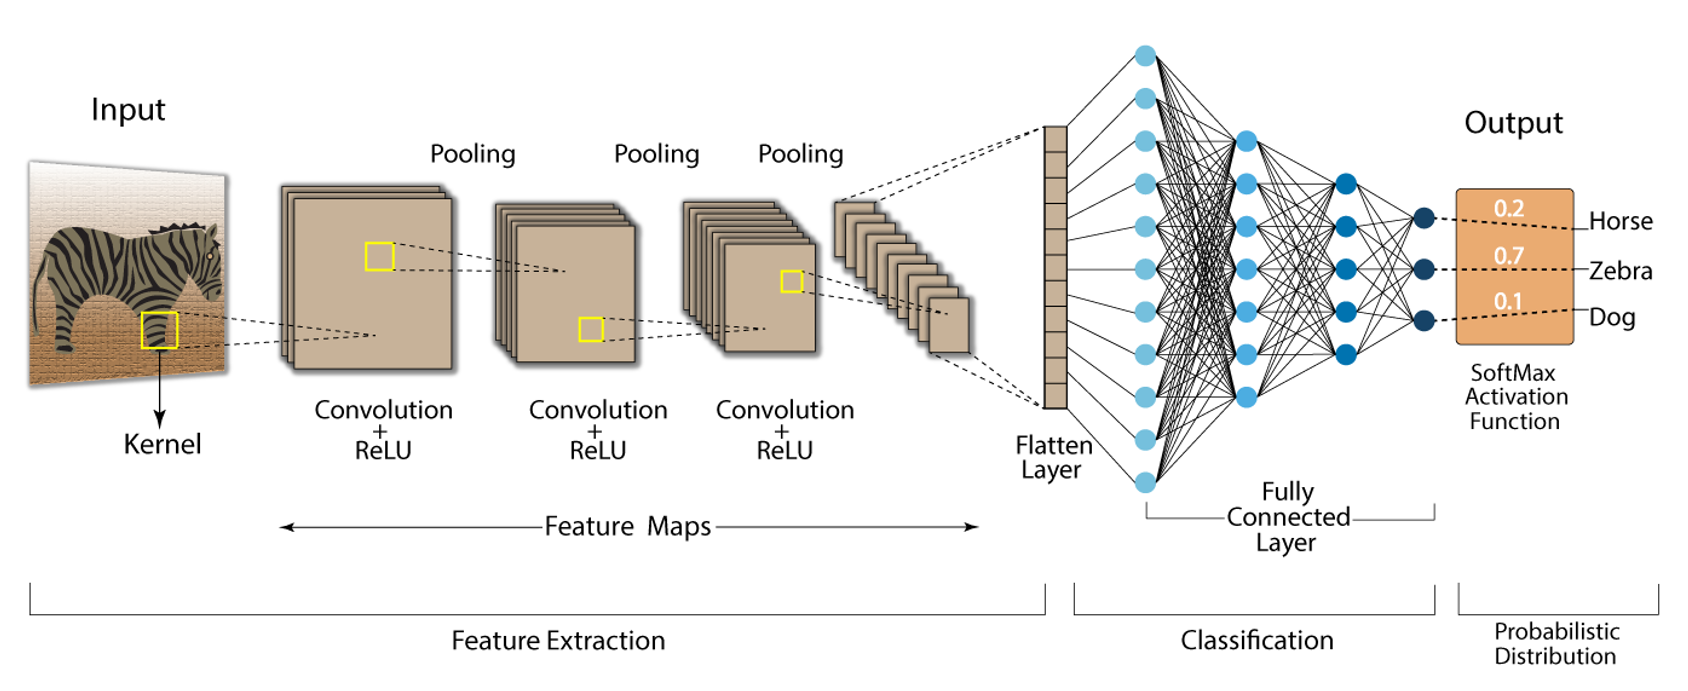
\includegraphics[width=\textwidth]{Images/overview_CNN.png}
    \caption[General structure of a convolutional neural network]{General structure of a convolutional neural network \cite{developersbreachCNN}}
    \label{fig:cnn-overview}
\end{figure}

Compared with a fully connected neural network, a CNN requires fewer parameters for image-related tasks because it uses local connectivity and weight sharing. In a fully connected layer, each output neuron is connected to all input elements, which leads to a very large number of parameters for high-resolution images. In contrast, a convolutional layer uses a small kernel that slides across the input feature map. The same kernel weights are reused at different spatial locations, enabling the network to detect similar features regardless of their positions in the image. This mechanism reduces memory requirements and improves generalization.

\subsubsection{Fundamental Layers in CNN Architecture}

A CNN is constructed from several types of layers. Each layer has a specific role in transforming the input data into useful feature representations. The most common components are convolutional layers, activation layers, pooling or down-sampling layers, and fully connected layers. In modern image compression and generative architectures, fully connected layers are often avoided or used only in small auxiliary networks because convolutional layers are more efficient for preserving spatial structure.

\paragraph{Convolutional Layer}

The convolutional layer is the main computational component of a CNN. Its purpose is to extract local features from the input by applying a set of learnable kernels. For an input feature map, each kernel scans over local receptive fields and produces one output feature map. When multiple kernels are used, the layer generates multiple output channels, where each channel corresponds to a different learned feature detector.

The convolution operation is illustrated in Figure~\ref{fig:cnn-convolutional-layer}. At each spatial position, the kernel values are multiplied by the corresponding input values, and the products are accumulated to form one output value. This multiply-accumulate pattern dominates the computational cost of CNN inference and is therefore a key target for hardware acceleration.

\begin{figure}[htbp]
    \centering
    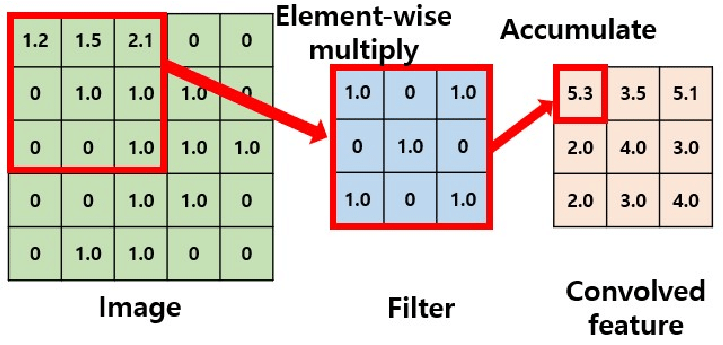
\includegraphics[width=0.82\textwidth]{Images/conv.png}
    \caption{Illustration of a convolution operation in a CNN layer}
    \label{fig:cnn-convolutional-layer}
\end{figure}

For a convolutional layer, the spatial size of the output feature map depends on the input size, kernel size, stride, and padding. If the input height and width are denoted by $H$ and $W$, the kernel height and width by $K_h$ and $K_w$, the padding by $P$, and the stride by $S$, then the output height $H_{out}$ and output width $W_{out}$ can be calculated as
\begin{equation}
H_{out} = \left\lfloor \frac{H - K_h + 2P}{S} \right\rfloor + 1,
\end{equation}
\begin{equation}
W_{out} = \left\lfloor \frac{W - K_w + 2P}{S} \right\rfloor + 1.
\end{equation}

Stride controls how far the kernel moves after each computation. A larger stride reduces the output resolution and decreases the number of operations. Padding adds values, usually zeros, around the input boundary so that border information can be included in the convolution. Padding is also used to preserve the spatial size of feature maps when necessary.

\paragraph{Activation Function}

A convolution operation is linear. Therefore, activation functions are inserted after convolutional layers to introduce nonlinearity into the network. Without nonlinear activation, a deep stack of convolutional layers would still be equivalent to a linear transformation and would have limited representational power. Common activation functions include Rectified Linear Unit (ReLU), sigmoid, hyperbolic tangent (tanh), and Swish.

ReLU is widely used because of its simple hardware-friendly computation and its ability to reduce the vanishing gradient problem. It is defined as
\begin{equation}
f(x) = \max(0, x).
\end{equation}

For more complex neural networks, other activation functions may be selected to improve accuracy or perceptual quality. In hardware implementation, the activation function must be considered carefully because nonlinear functions such as sigmoid or Swish are more expensive to implement than ReLU. For a quantized accelerator, this issue becomes even more important because the activation function must be compatible with fixed-point arithmetic and efficient lookup or approximation methods.

\paragraph{Pooling and Down-Sampling Layers}

Pooling layers reduce the spatial size of feature maps, which lowers computational complexity and decreases memory usage. In particular, max pooling selects the largest activation within each local window, producing a down-sampled feature map while preserving the most salient features from the input region. Figure~\ref{fig:max-pooling} illustrates this process: each pooling window is replaced by its maximum value, so the output feature map retains strong responses while its spatial dimensions are reduced.

\begin{figure}[htbp]
    \centering
    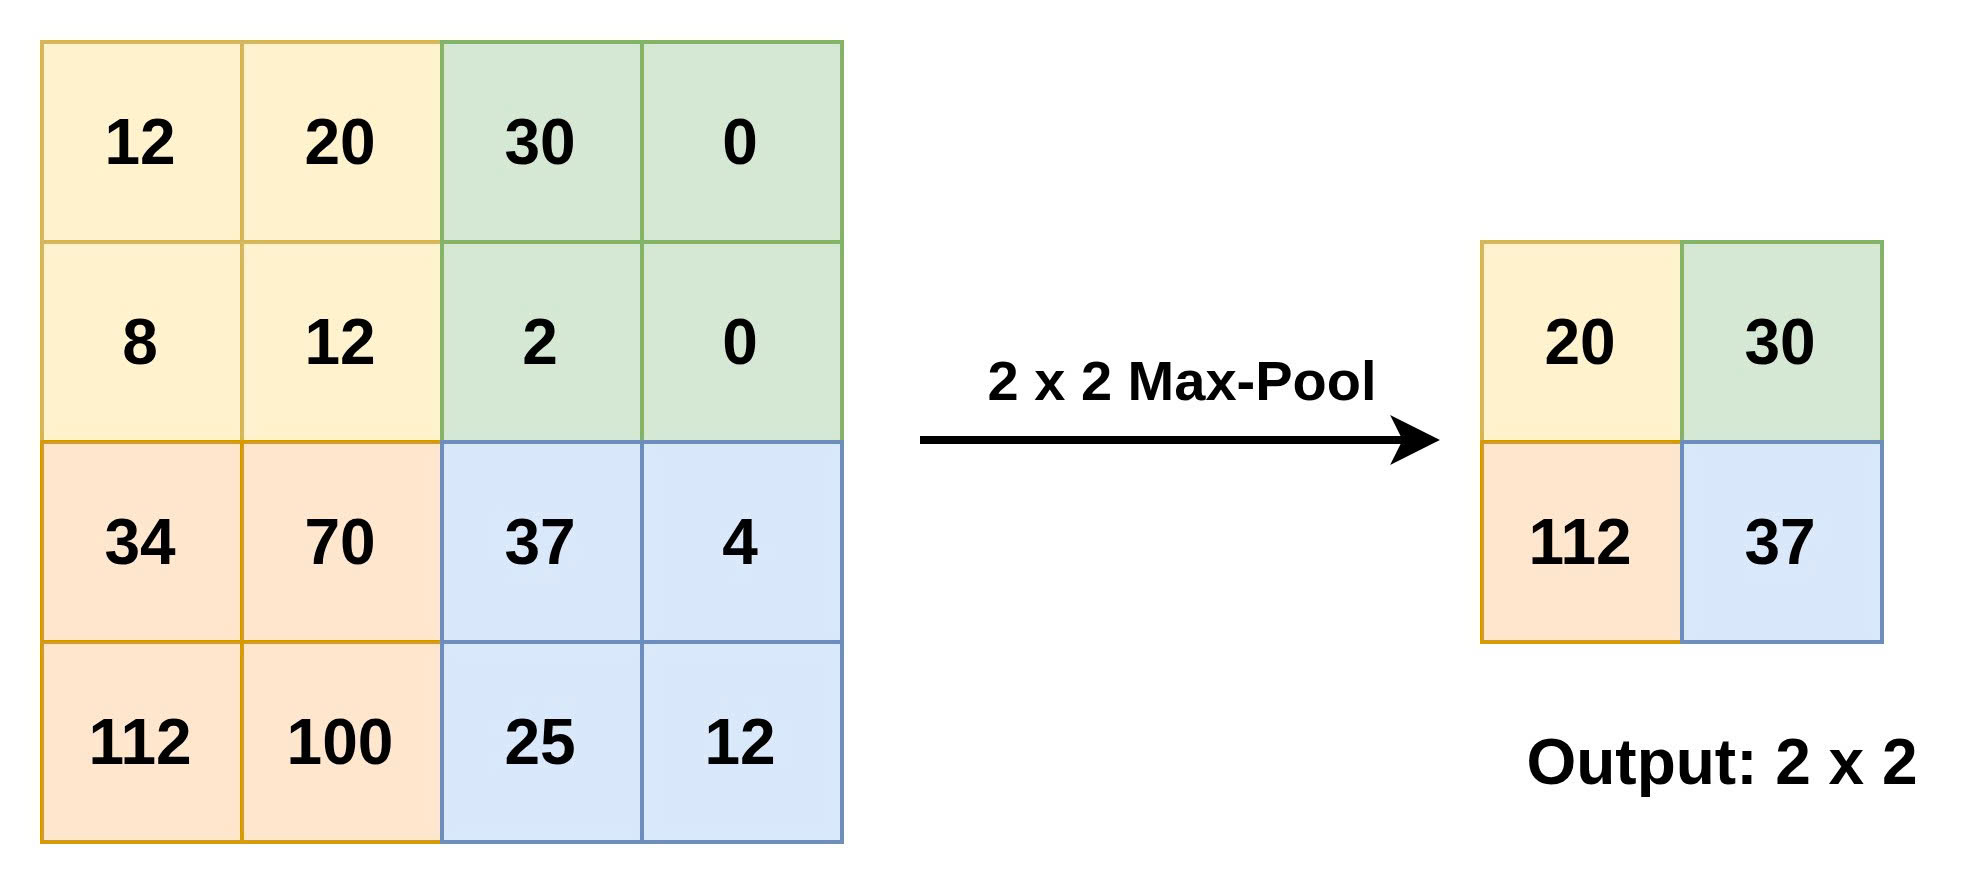
\includegraphics[width=0.72\textwidth]{Images/max_pooling.jpg}
    \caption{Max pooling.}
    \label{fig:max-pooling}
\end{figure}

Average pooling is another common method, but in image-compression and generative models, max pooling is often preferred when the goal is to preserve strong feature responses. In many modern CNN-based compression and generation models, down-sampling may also be performed by strided convolution instead of a separate pooling layer. Strided convolution has learnable parameters, so it can reduce resolution while also extracting features. This approach is useful in encoder networks, where the image must be transformed into a lower-resolution latent representation.

\paragraph{Normalization Layer}

Normalization layers rescale intermediate feature maps to a consistent statistical range, which stabilizes and accelerates training. Common variants include batch normalization, instance normalization, and channel (layer) normalization, which differ in the dimensions over which the mean and variance are computed. For a feature value $x$, normalization can be expressed as
\begin{equation}
\hat{x} = \gamma \cdot \frac{x - \mu}{\sqrt{\sigma^2 + \epsilon}} + \beta,
\end{equation}
where $\mu$ and $\sigma^2$ are the mean and variance computed over the chosen dimensions, $\epsilon$ is a small constant for numerical stability, and $\gamma$ and $\beta$ are learnable scale and shift parameters. The HiFiC generator applies channel normalization inside its residual blocks, so each residual block contains convolution, normalization, and activation. In a quantized hardware implementation, normalization must be handled carefully because its division and square-root operations are more expensive than multiply-accumulate and are sensitive to reduced precision.

\paragraph{Residual Connections}

As illustrated in Figure~\ref{fig:residual-connection}, a residual connection adds the input of a block directly to its output through a skip path, so that the convolutional path only has to learn a residual mapping $F(x)$ instead of a full transformation:
\begin{equation}
y = x + F(x),
\end{equation}
where $x$ is the input feature map and $F(x)$ is the transformation produced by the convolutional path. Residual connections improve gradient flow and feature reuse, which makes deep networks easier to train.

\begin{figure}[htbp]
    \centering
    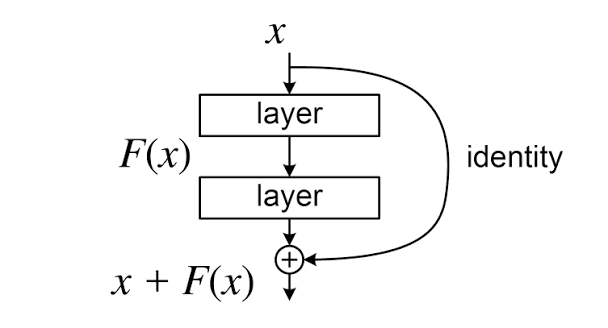
\includegraphics[width=0.72\textwidth]{Images/residual_connection.png}
    \caption{Residual connection}
    \label{fig:residual-connection}
\end{figure}

The building block that implements this pattern is called a residual block (ResBlock). In the HiFiC generator, the ResBlock combines convolution, normalization, activation, and a skip connection, and is repeated many times. Because these repeated ResBlocks dominate the inference computation, they are the main target for hardware acceleration in this thesis.

\paragraph{Transposed Convolution and Up-Sampling}

While the encoder reduces spatial resolution, the generator must increase resolution to reconstruct the output image. This is achieved by up-sampling operations, most commonly transposed convolution (also called deconvolution or fractionally-strided convolution)~\cite{huytran2021transposedconv}. Whereas a normal convolution performs a many-to-one mapping that aggregates a local input window into a single output value, transposed convolution performs the inverse one-to-many mapping: each input value is multiplied by the entire kernel and its contribution is spread across a neighbourhood of output positions, thereby expanding the feature map. It provides a \emph{learnable} up-sampling, in contrast to fixed methods such as nearest-neighbor or bilinear interpolation.

For an input of size $i$, kernel size $k$, stride $s$, and padding $p$, the output size of a transposed convolution is
\begin{equation}
o = (i - 1)\,s + k - 2p .
\end{equation}
Unlike the normal convolution formula, no floor operation appears because the stride multiplies the spacing between projected input samples instead of dividing the input size; a stride $s>1$ therefore \emph{increases} the output resolution. In the HiFiC generator, several up-convolution blocks each apply a $3\times3$ transposed convolution with stride two, progressively restoring the spatial resolution of the latent representation back to the original image size.

In practice, deep-learning frameworks compute a transposed convolution by reducing it to an ordinary convolution, as illustrated in Figure~\ref{fig:transposed_conv_steps}. Starting from the stride $s$ and padding $p$, the input is first expanded by inserting $z = s-1$ zeros between adjacent rows and columns; a border of $p' = k-p-1$ zeros is then added around the expanded input; finally a standard convolution with unit stride is slid over the result to produce the up-sampled output. This zero-insertion procedure is what allows a network to learn the up-sampling weights while reusing a conventional convolution operator.

\begin{figure}[H]
    \centering
    
\includegraphics[width=\textwidth]{Images/transposed_conv_steps.png}
    \caption[Four-step computation of a transposed convolution]{Four-step computation of a transposed convolution \cite{huytran2021transposedconv}}
    \label{fig:transposed_conv_steps}
\end{figure}

\paragraph{Scatter and Gather Views of Transposed Convolution}

Transposed convolution can be computed in two mathematically equivalent ways, illustrated in Figure~\ref{fig:scatter_gather}.

In the \textbf{scatter} view (top of Figure~\ref{fig:scatter_gather}), the operation follows its natural definition. Each input pixel is multiplied by every kernel tap, producing a weighted copy of the kernel that is placed (scattered) onto the output grid at a position determined by the stride. Because the strided placements of neighbouring input pixels overlap, output positions that receive contributions from several input pixels are summed. A single output pixel is therefore written several times and is only complete after all input pixels have scattered their contributions, which requires an accumulation buffer over the output.

In the \textbf{gather} view (bottom of Figure~\ref{fig:scatter_gather}), the same result is obtained by reducing the problem to a standard convolution: zeros are inserted between the input samples (and around the border) according to the stride, the kernel is flipped ($180^\circ$ rotation), and an ordinary stride-one convolution is then applied to the zero-expanded input. Each output pixel now gathers a fixed local window, exactly as in a normal convolution. This view is convenient for analysis and for reusing a standard convolution engine, but the inserted zeros lead to wasted multiplications.

\begin{figure}[H]
    \centering
    
\includegraphics[width=0.82\textwidth]{Images/Scatter_Gather.png}
    \caption{Scatter and gather views of a $2\times2$ transposed convolution with stride two}
    \label{fig:scatter_gather}
\end{figure}

The choice between the scatter and gather formulations directly shapes the hardware design of the up-convolution accelerator presented in \hyperref[chap:implementation]{Chapter~3}: the scatter formulation avoids the wasted multiplications of the zero-inserted gather formulation, but in exchange requires a row-wide accumulation buffer because each output pixel is updated several times.

\subsubsection{Advantages and Limitations of CNNs for Hardware Acceleration}

CNNs have several advantages for hardware implementation. First, convolution operations contain a high degree of data reuse. The same weights are applied to many spatial positions, and neighboring output pixels often share overlapping input windows. This reuse can be exploited through on-chip buffers and parallel processing elements. Second, CNN layers are highly parallel because many output pixels and output channels can be computed independently. This parallelism is suitable for FPGA and ASIC accelerators. Third, CNN models can be optimized using quantization, pruning, and layer fusion to reduce computation and memory traffic.

However, CNNs also create several hardware challenges. Deep CNNs require a large number of multiply-accumulate operations, which may exceed the capability of general-purpose processors when real-time performance is required. In addition, feature maps and model weights can occupy significant memory, leading to high bandwidth demand between external memory and the accelerator. Some layers, such as normalization and complex activation functions, may have irregular access patterns or nonlinear operations that are less straightforward to accelerate.

For the quantized HiFiC GAN accelerator in this thesis, these advantages and limitations motivate a hardware-software co-design approach. The software side is responsible for model preparation, quantization, parameter management, and system control, while the hardware side accelerates the dominant CNN computations. By designing both sides together, the system can better satisfy the requirements of learned image compression, including high throughput, reduced resource usage, and acceptable reconstructed image quality.

\subsection{Generative Adversarial Networks}

Generative Adversarial Networks (GANs) are a class of generative models designed to learn the distribution of real data and synthesize new samples that appear realistic. A typical GAN consists of two neural networks trained in competition: a generator and a discriminator. The generator attempts to produce data samples that resemble the training distribution, while the discriminator attempts to distinguish generated samples from real samples. Through this adversarial training process, the generator gradually improves its ability to create outputs that are visually plausible. \cite{goodfellow2014gan}

In image-related applications, GANs are particularly useful because they can encourage outputs to match the perceptual characteristics of natural images rather than only minimizing pixel-wise error. This is important because traditional distortion metrics, such as Mean Squared Error (MSE), often favor overly smooth reconstructions when the compression ratio is high. Although such reconstructions may achieve acceptable numerical distortion, they can lose fine textures and perceptually important details. GAN-based objectives address this limitation by comparing the distribution of reconstructed images with the distribution of real images, thereby improving perceptual realism. \cite{blau2018perception,mentzer2020high}

The use of GANs in learned image compression is motivated by the rate--distortion--perception trade-off. At a fixed bitrate, optimizing only distortion does not necessarily lead to the best perceptual quality. Conversely, improving perceptual quality may increase the measured distortion between the original and reconstructed images. Therefore, GAN-based compression methods introduce an adversarial loss to guide the reconstruction toward the natural image manifold. This makes the reconstructed image visually more convincing, especially at low bitrates where classical codecs may produce blocking or banding artifacts and distortion-optimized neural codecs may produce blur. \cite{blau2018perception,mentzer2020high}

However, GAN-based compression models also introduce implementation challenges. The generator network usually contains many convolutional and residual blocks, which require substantial multiply-accumulate operations and memory bandwidth during inference. In addition, the numerical behavior of a GAN-based decoder can be sensitive to quantization because small changes in intermediate feature maps may affect perceptual details in the reconstructed image. These characteristics motivate a hardware-software co-design approach, where software handles model preparation and system control while hardware accelerates the most computationally intensive neural network blocks. \cite{mentzer2020high,sze2017efficient}

\subsection{HiFiC GAN Architecture for Learned Image Compression}

High-Fidelity Image Compression (HiFiC) is a GAN-based learned image compression framework that combines neural compression with adversarial learning to improve perceptual reconstruction quality. Instead of optimizing only for pixel-wise similarity, HiFiC aims to reconstruct images that are visually close to the input while maintaining practical bitrates. The original HiFiC study showed that GAN-based compression can produce high-fidelity reconstructions and can be evaluated using both perceptual metrics and human preference studies. \cite{mentzer2020high}

The overall HiFiC architecture used in this thesis can be divided into three main components: an encoder network, a hyperprior network, and a generator network, as shown in Figure~\ref{fig:hific-architecture}. The encoder transforms the input RGB image into a compact latent representation. This latent representation contains the information required for reconstruction while removing spatial redundancy from the input image. The hyperprior network models the statistical distribution of the latent variables and provides side information for more efficient entropy coding. Finally, the generator reconstructs the image from the compressed latent representation. \cite{mentzer2020high,balle2018variational}

\begin{figure}[htbp]
    \centering
    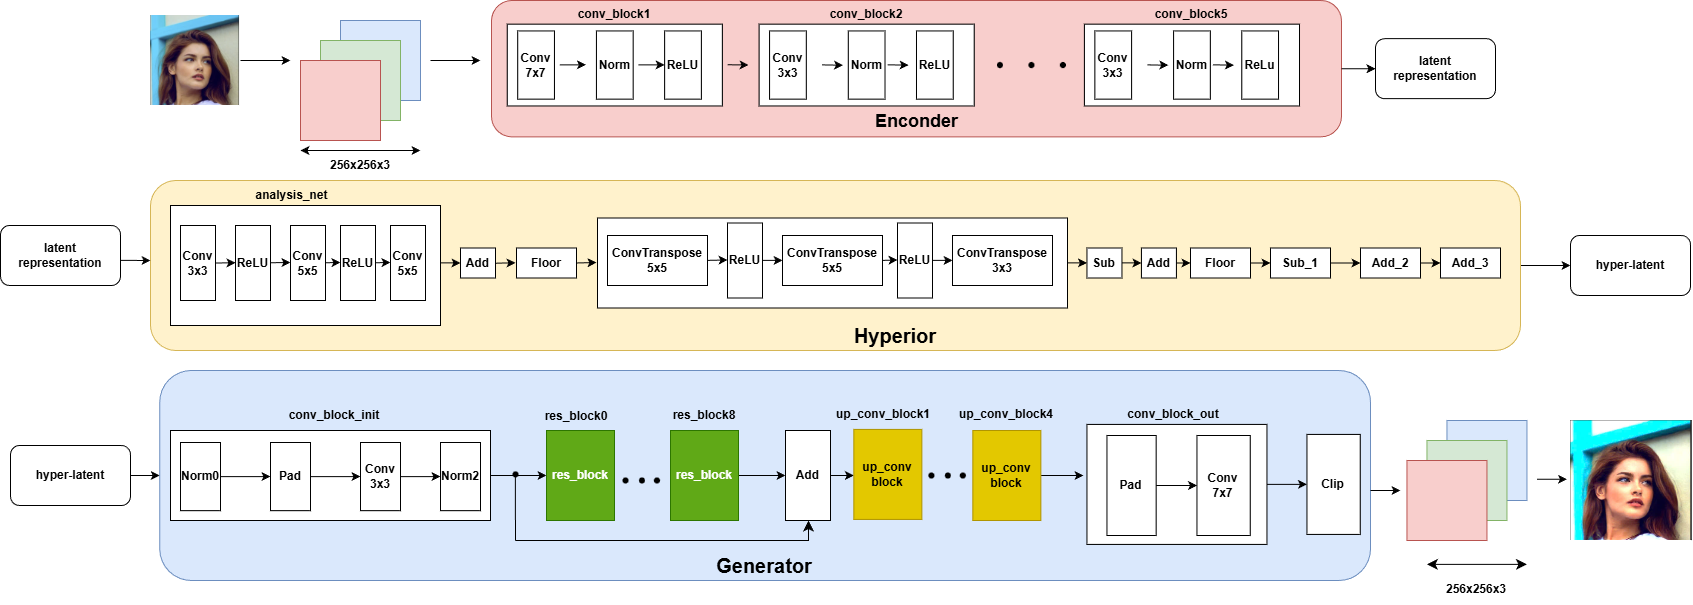
\includegraphics[width=\textwidth]{Images/HiFiC.png}
    \caption{Overview of the HiFiC GAN-based learned image compression architecture}
    \label{fig:hific-architecture}
\end{figure}

The encoder is implemented as a sequence of convolutional blocks. Each block extracts hierarchical image features while reducing redundancy in the spatial domain. Unlike a conventional autoencoder trained only with a pixel-wise loss, the HiFiC encoder is optimized as part of a perceptual compression system. As a result, the latent representation is expected to preserve visually meaningful information that supports high-quality reconstruction at the decoder side. \cite{mentzer2020high}

The hyperprior network improves compression efficiency by learning side information about the latent representation. This side information, often called hyper-latent variables, helps estimate the entropy model used for coding the compressed representation. A more accurate entropy model allows the system to assign shorter codes to more likely latent symbols, which reduces bitrate while maintaining reconstruction quality. \cite{balle2018variational}

The generator network is responsible for reconstructing the output image from the latent and hyper-latent information. In the HiFiC generator design, the generator contains an initial convolutional block, multiple residual blocks, reconstruction blocks, and a final convolutional block. The residual blocks include convolution, normalization, activation functions, and skip connections. These skip connections improve feature reuse and help stabilize the reconstruction process. Because residual blocks contain repeated convolution-heavy operations, they dominate the computational workload and become a natural target for hardware acceleration. \cite{mentzer2020high,sze2017efficient}

For the hardware-software co-design in this thesis, the generator is selected as the primary acceleration target because it contains most of the inference-time computation. The remaining components can be executed in software to preserve flexibility in model control, data formatting, and system integration. This partitioning provides a practical balance between hardware efficiency and software programmability, which is important for deploying a quantized HiFiC model on FPGA-based embedded platforms. \cite{mentzer2020high,sze2017efficient}

\subsection{Quantization and Numerical Precision}

Neural networks are typically trained using 32-bit floating-point (FP32) arithmetic, which provides high numerical precision but is expensive in terms of memory footprint, memory bandwidth, and arithmetic resource usage. Quantization reduces the numerical precision of weights and activations to a lower-bit representation so that the model requires less storage and can be executed with smaller, faster arithmetic units. This is particularly important for FPGA deployment, where on-chip memory and DSP resources are limited.

Quantization methods are generally divided into two categories. Quantization-aware training (QAT) simulates reduced precision during training so that the model can adapt to quantization noise, whereas post-training quantization (PTQ) converts an already trained FP32 model to lower precision without retraining. PTQ is faster to deploy and is the approach adopted in this thesis.

The numerical format also matters. Integer formats such as INT8 offer the smallest footprint but have a limited dynamic range, which can be problematic for GAN-based decoders where small numerical errors may produce visible artifacts. Half-precision floating-point (FP16) keeps a floating-point exponent, so it preserves a wider dynamic range than integer formats while still halving the storage and increasing the arithmetic density compared with FP32. For this reason, the proposed accelerator adopts a mixed-precision scheme in which the input and output interfaces remain in FP32 for compatibility, while the internal computation of the generator is performed in FP16. The detailed quantization strategy applied to the HiFiC model is presented in Chapter~3.



\subsection{Evaluation Metrics for GAN Accelerator and Image Compression}

Evaluation metrics are required to assess both the hardware efficiency of the proposed GAN accelerator and the reconstruction quality of the learned image compression model. Since this thesis focuses on a quantized HiFiC GAN accelerator, the evaluation should consider two complementary aspects. The first aspect measures how efficiently the accelerator executes the neural network workload on hardware. The second aspect measures how close the reconstructed image is to the original image after compression and decompression.

\subsubsection{Metrics for GAN Accelerator}

The performance of a GAN accelerator can be evaluated using several hardware-oriented metrics. These metrics are adapted from common CNN accelerator evaluation criteria because the generator network in HiFiC is mainly composed of convolutional and residual blocks. Therefore, latency, throughput, inference speed, power consumption, power efficiency, and FPGA resource utilization are important indicators for analyzing the efficiency of the proposed design. \cite{sze2017efficient}

Latency measures the time required by the accelerator to process one input image and produce the corresponding reconstructed output. In real-time or near-real-time image compression systems, lower latency is desirable because it reduces the waiting time between input acquisition and output reconstruction. If the accelerator requires $n_T$ clock cycles and the clock period is $T$, the latency can be written as
\begin{equation}
Latency = n_T \times T.
\end{equation}
Since the clock period is the inverse of the operating frequency $F$, the latency can also be expressed as
\begin{equation}
Latency = \frac{n_T}{F}.
\end{equation}

Throughput represents the amount of computation completed per second. For neural network accelerators, it is commonly expressed in Giga Operations Per Second (GOPS). A higher throughput indicates that the hardware can process more arithmetic operations in a fixed time interval. If the computational workload of the model is denoted by $Workload$ in GOPs, the throughput is calculated as
\begin{equation}
Throughput~(GOPS) = \frac{Workload~(GOPs)}{Latency~(s)}.
\end{equation}

Inference speed describes how many images or frames can be processed per second. It is usually measured in frames per second (fps). For an image compression accelerator, this metric indicates how many reconstructed images can be generated in one second. The inference speed is the inverse of latency:
\begin{equation}
Inference~Speed~(fps) = \frac{1}{Latency~(s)}.
\end{equation}

Power consumption is another important metric, especially for FPGA-based embedded systems. It indicates the amount of electrical power consumed by the accelerator during execution. The total power may include the power used for computation, on-chip memory access, external memory transfer, control logic, and input/output interfaces. Lower power consumption is beneficial for portable or energy-constrained systems.

Power efficiency evaluates how much computational performance is achieved for each watt of power. It is calculated as the ratio between throughput and power consumption:
\begin{equation}
Power~Efficiency~(GOPS/W) = \frac{Throughput~(GOPS)}{Power~Consumption~(W)}.
\end{equation}
A higher value means that the accelerator can deliver more computation with less energy, which is desirable for practical deployment.

Resource utilization is used to analyze how much of the FPGA fabric is occupied by the accelerator. The main resource metrics include logic utilization, DSP utilization, and BRAM utilization. Logic utilization reflects the amount of configurable logic used for control and data-path implementation. DSP utilization shows how many dedicated arithmetic blocks are used for multiply-accumulate operations. BRAM utilization indicates the amount of on-chip memory used for storing input feature maps, intermediate feature maps, weights, and temporary buffers. These metrics help determine whether the accelerator is compact, scalable, and suitable for the target FPGA platform.

\subsubsection{Metrics for Image Compression}

In addition to hardware metrics, image compression quality must be evaluated by comparing the reconstructed image with the original image. Two commonly used objective metrics are Peak Signal-to-Noise Ratio (PSNR) and Structural Similarity Index Measure (SSIM). PSNR measures pixel-wise reconstruction fidelity, while SSIM evaluates structural similarity from a perceptual perspective. \cite{huynh2008scope,wang2004ssim}

PSNR is derived from the Mean Squared Error (MSE) between the original image and the reconstructed image. For an image with height $H$, width $W$, and $C$ color channels, the MSE is defined as
\begin{equation}
MSE = \frac{1}{HWC}\sum_{i=1}^{H}\sum_{j=1}^{W}\sum_{k=1}^{C}\left(I(i,j,k)-\hat{I}(i,j,k)\right)^2,
\end{equation}
where $I$ is the original image and $\hat{I}$ is the reconstructed image. PSNR is then computed as
\begin{equation}
PSNR = 10\log_{10}\left(\frac{MAX_I^2}{MSE}\right),
\end{equation}
where $MAX_I$ is the maximum possible pixel value. For 8-bit images, $MAX_I = 255$. A higher PSNR generally indicates lower pixel-level distortion and better reconstruction fidelity.

SSIM measures the similarity between two images by comparing luminance, contrast, and structural information. For two image patches $x$ and $y$, SSIM is commonly expressed as
\begin{equation}
SSIM(x,y) = \frac{(2\mu_x\mu_y + C_1)(2\sigma_{xy} + C_2)}{(\mu_x^2 + \mu_y^2 + C_1)(\sigma_x^2 + \sigma_y^2 + C_2)},
\end{equation}
where $\mu_x$ and $\mu_y$ are the mean intensities, $\sigma_x^2$ and $\sigma_y^2$ are the variances, $\sigma_{xy}$ is the covariance between $x$ and $y$, and $C_1$, $C_2$ are small constants used to avoid numerical instability. SSIM values are usually in the range from 0 to 1, where a value closer to 1 indicates higher structural similarity.

For the quantized HiFiC GAN accelerator, PSNR and SSIM provide useful objective indicators of reconstruction quality after quantization and hardware-oriented optimization. However, because GAN-based compression is designed to improve perceptual quality, these metrics should be interpreted together with perceptual evaluation and visual comparison. A reconstruction with slightly lower PSNR may still appear more natural if it preserves textures and perceptual details better than a distortion-optimized reconstruction. \cite{blau2018perception,mentzer2020high,huynh2008scope,wang2004ssim}

\subsection{Hardware Platform}

The proposed accelerator is intended to be deployed on a Field-Programmable Gate Array (FPGA) platform. An FPGA is an integrated circuit that can be configured after manufacturing to implement a specific digital system. Unlike CPUs and GPUs, which execute instructions on a fixed architecture, an FPGA allows the designer to customize the hardware datapath, memory organization, and control logic according to the target algorithm. This flexibility makes FPGAs suitable for accelerating neural network workloads that require high parallelism, low latency, and efficient energy usage. \cite{kuon2008fpga,sze2017efficient}

An FPGA device is mainly composed of configurable logic blocks, programmable interconnects, on-chip memory resources, and dedicated arithmetic units. Configurable logic blocks are used to implement control circuits and custom datapaths. Programmable interconnects connect these logic blocks and allow the designer to build a complete hardware architecture. On-chip memory blocks, commonly referred to as Block RAM (BRAM), store intermediate feature maps, weights, partial sums, and temporary buffers. Dedicated Digital Signal Processing (DSP) slices are optimized for arithmetic operations such as multiplication and accumulation, which are dominant in convolutional neural networks and GAN generators.

For deep neural network acceleration, FPGAs provide several important advantages. First, they support fine-grained parallelism, allowing multiple processing elements to operate at the same time. This property is useful for convolutional and residual blocks, where many output pixels and channels can be computed independently. Second, FPGAs allow customized dataflow architectures that can increase data reuse and reduce external memory access. Since memory transfer often consumes significant energy and limits performance, keeping frequently used data in on-chip buffers is important for efficient accelerator design. Third, FPGAs can support different numerical precisions, such as fixed-point, integer, or floating-point formats, making them suitable for quantized neural network implementation.

In the context of the quantized HiFiC GAN accelerator, the FPGA platform is used to accelerate the computationally intensive generator network. The generator contains repeated convolutional and residual operations that can benefit from parallel multiply-accumulate units, pipelined execution, and local buffering. By mapping these operations to FPGA resources, the system can reduce inference latency and improve energy efficiency compared with executing the entire model on a general-purpose processor.

However, FPGA implementation also introduces several design constraints. The available number of logic elements, DSP slices, and BRAM blocks is limited, so the accelerator architecture must be carefully optimized to fit the target device. In addition, the memory bandwidth between external memory and the FPGA fabric can become a bottleneck if feature maps and weights are transferred frequently. Therefore, an efficient FPGA-based accelerator must balance parallelism, resource utilization, memory access, and operating frequency.

For this thesis, the hardware platform provides the physical foundation for hardware-software co-design. The software side prepares input data, controls execution, and manages communication with memory, while the FPGA accelerator performs the most time-consuming neural network computations. This division enables the system to preserve software flexibility while exploiting hardware-level parallelism for the quantized HiFiC GAN workload.


\subsection{High-Level Synthesis}

High-Level Synthesis (HLS) is an automated design process that converts a behavioral description written in C/C++ or SystemC into a register-transfer level (RTL) hardware implementation. According to the Vitis HLS user guide, the HLS flow starts from an algorithmic description, verifies it at C level, synthesizes RTL under clock and design constraints, verifies the generated RTL, and allows multiple architectures to be explored from the same source code \cite{amd2026vitisHls}.

\subsubsection{Why HLS is Used}

The main motivation for using HLS in this thesis is productivity. A ResBlock contains nested loops, convolution windows, channel accumulation, normalization, activation, and residual addition. Writing all these components directly in Verilog would require manual finite-state machines, address generators, pipeline registers, memory controllers, and interface logic. HLS allows the algorithm to be described closer to the C/C++ implementation, while pragmas guide the tool to generate the desired hardware micro-architecture.

Fig.~\ref{fig:ug1399_hls_steps} illustrates the main steps of HLS. The tool compiles the algorithm, schedules operations into clock cycles, binds operations to hardware resources, generates RTL, and then passes the design to logic synthesis. The important point is that HLS does not remove the need for hardware thinking. The designer still has to define the macro-architecture, memory hierarchy, parallelism, and interface protocol. Pragmas are the bridge between the algorithmic C/C++ description and the hardware architecture expected by the designer.

\begin{figure}[H]
    \centering
    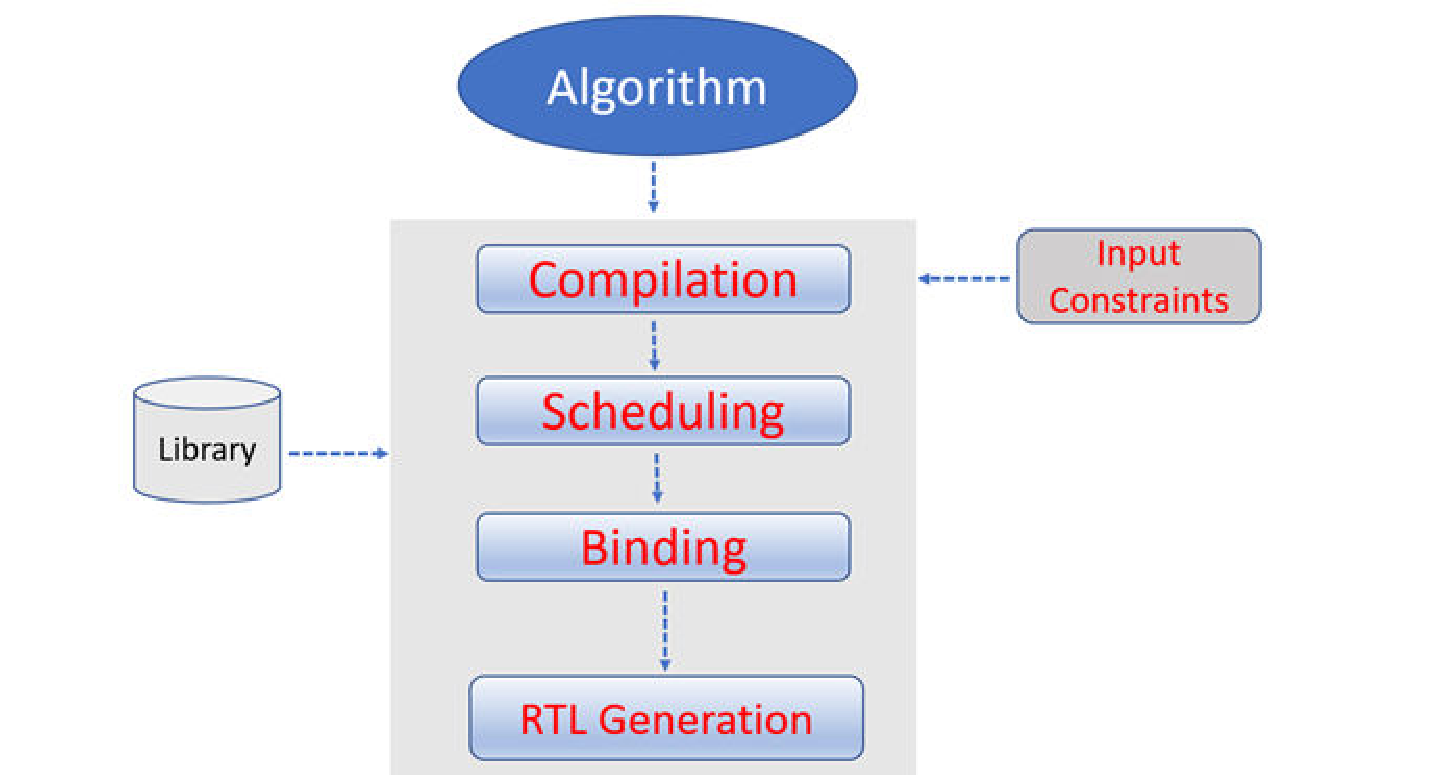
\includegraphics[width=0.78\textwidth]{Images/ug1399_hls_steps.png}
    \caption[HLS compilation, scheduling, binding, and RTL generation flow]{HLS compilation, scheduling, binding, and RTL generation flow \cite{amd2026vitisHls}}
    \label{fig:ug1399_hls_steps}
\end{figure}

Compared with traditional handwritten Verilog or VHDL, HLS provides a faster design-space exploration loop. The same C/C++ source can generate different RTL implementations by changing pragmas and constraints. This is valuable for CNN accelerators because the designer often has to trade latency against resource utilization. For example, increasing the unroll factor improves parallelism but consumes more DSP and LUT resources. Partitioning arrays improves memory bandwidth but consumes more BRAMs or registers.

\begin{table}[H]
\centering
\caption{Comparison between HLS-based design and traditional handwritten RTL design}
\label{tab:hls_vs_rtl}
\begin{tabularx}{\textwidth}{|p{0.23\textwidth}|X|X|}
\hline
\textbf{Aspect} & \textbf{HLS-based design} & \textbf{Handwritten Verilog/VHDL} \\
\hline
Design entry & C/C++ algorithm with hardware-aware coding style and pragmas & Cycle-level RTL modules, FSMs, registers, and datapaths written manually \\
\hline
Development speed & Faster algorithm iteration and verification at C level & Slower but gives full control over every clock cycle and signal \\
\hline
Architecture exploration & Pragmas and constraints can generate multiple implementations from one source & Architecture changes often require significant RTL rewriting \\
\hline
Micro-architecture control & Controlled indirectly through scheduling, binding, interfaces, and memory pragmas & Controlled explicitly by the designer \\
\hline
Best suited for & Algorithm-dominated kernels such as convolution, filters, and dataflow pipelines & Highly specialized control paths, custom protocols, or manually optimized low-level blocks \\
\hline
\end{tabularx}
\end{table}

\subsubsection{Scheduling, Binding, and Generated Circuit Structure}

HLS transforms an untimed C/C++ description into a timed RTL circuit through scheduling and binding. Scheduling determines which operations execute in each clock cycle based on data dependencies, clock period, resource availability, and user directives. Binding maps scheduled operations to concrete hardware resources such as DSP blocks, LUT-based adders, memories, multiplexers, and registers \cite{amd2026vitisHls}.

Fig.~\ref{fig:ug1399_scheduling_binding} shows a simplified scheduling and binding example. At the C level, the expression is written as ordinary arithmetic. During scheduling, the operations are assigned to clock cycles. During binding, multiplication and addition are mapped to functional units such as DSP or AddSub blocks. This is exactly where HLS pragmas affect the generated circuit: a pipeline pragma changes the timing schedule, an unroll pragma changes how many copies of the datapath are created, an array partition pragma changes the memory structure, and a bind operation pragma changes the resource selected for arithmetic.

\begin{figure}[H]
    \centering
    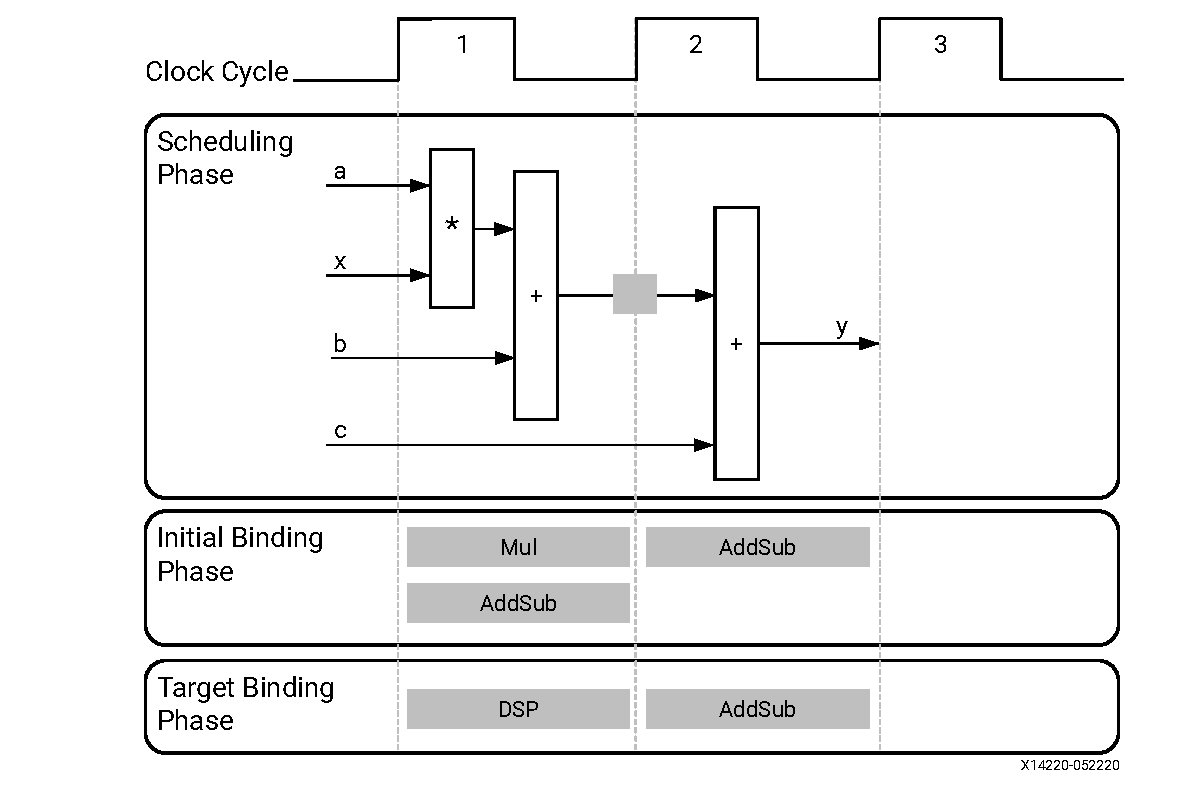
\includegraphics[width=0.82\textwidth]{Images/ug1399_scheduling_binding.png}
    \caption[Scheduling and binding example]{Scheduling and binding example \cite{amd2026vitisHls}}
    \label{fig:ug1399_scheduling_binding}
\end{figure}

For the HiFiC GAN ResBlock, this means the HLS code must be written with the final hardware in mind. The inner MAC loops should become pipelined datapaths. Channel or PE loops should become multiple parallel lanes. Buffers must provide enough memory ports to feed those lanes. Arithmetic operators should map to DSP blocks with predictable latency. The top-level function must expose AXI interfaces for PS--PL integration. Finally, the convolution pass and post-processing pass should overlap when possible.

\subsubsection{Pipeline Pragma}

The \texttt{\#pragma HLS PIPELINE} directive reduces the initiation interval of a loop or function by allowing operations from different loop iterations to execute concurrently. Without pipelining, a loop iteration must complete before the next iteration starts. With pipelining, the loop is divided into stages separated by registers. After the pipeline is filled, a new iteration can begin every II cycles. When \texttt{II=1} is achieved, the loop accepts new input every clock cycle.

Fig.~\ref{fig:ug1399_loop_pipeline} demonstrates this timing change. Without loop pipelining, read, compute, and write operations are serialized across iterations. With loop pipelining, these operations overlap, reducing the interval between consecutive reads from three cycles to one cycle in the illustrated example \cite{amd2026vitisHls}.

\begin{figure}[H]
    \centering
    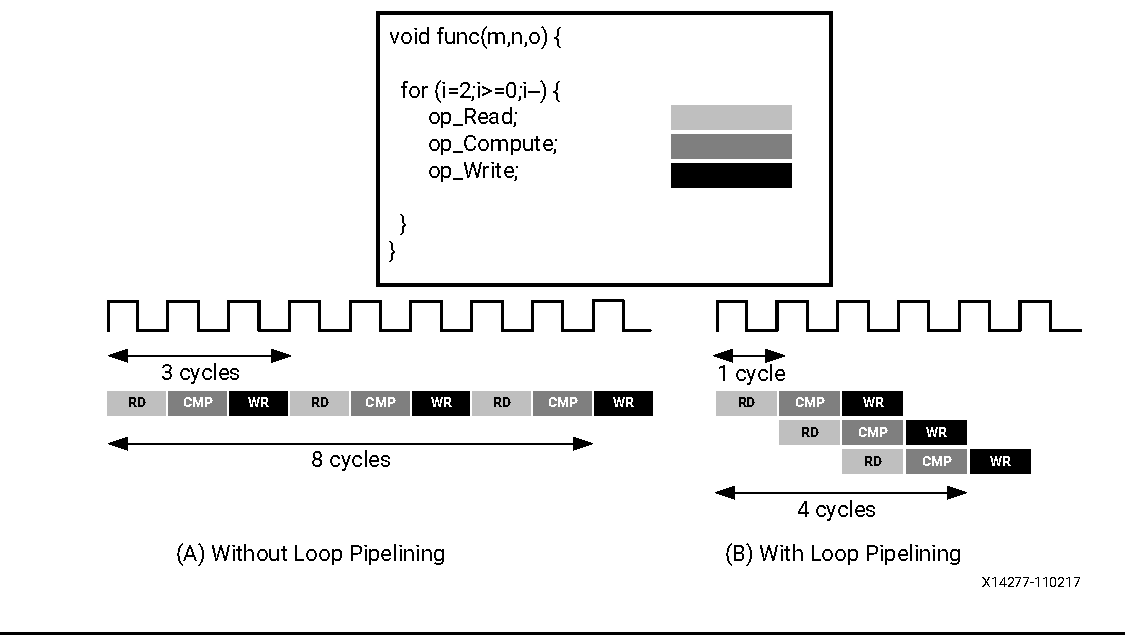
\includegraphics[width=0.82\textwidth]{Images/ug1399_loop_pipeline.png}
    \caption[Loop pipeline timing example]{Loop pipeline timing example \cite{amd2026vitisHls}}
    \label{fig:ug1399_loop_pipeline}
\end{figure}

In the proposed ResBlock, \texttt{PIPELINE II=1} is used for inner MAC loops inside each PE. At the circuit level, this creates pipeline registers along the multiplication and accumulation path and schedules the datapath so that different convolution windows are processed in overlapped clock cycles. The timing benefit is higher throughput: after the initial latency, the PE can produce one partial or final result per cycle if memory ports and dependencies do not stall the loop. This pragma is therefore most suitable for loops with regular data access and high iteration counts, such as convolution accumulation.

\subsubsection{Unroll Pragma}

The \texttt{\#pragma HLS UNROLL} directive transforms a loop by creating multiple copies of the loop body in hardware. If the loop is fully unrolled, all iterations are implemented as parallel hardware. If a factor $N$ is specified, $N$ copies of the loop body are created and the number of sequential loop iterations is reduced accordingly \cite{amd2026vitisHls}.

The hardware effect of partial loop unrolling is illustrated in Listings~\ref{lst:hls_unroll_original} and~\ref{lst:hls_unroll_exit_check}. A rolled loop reuses one datapath across multiple cycles, while an unrolled loop replicates the loop body so that several iterations can execute in parallel. The unroll factor does not have to be an integer divisor of the maximum loop iteration count. Therefore, when the trip count is not known exactly, Vitis HLS adds an exit check to preserve the same functionality as the original loop.

\begin{lstlisting}[caption={Pseudo-code before partial loop unrolling},label={lst:hls_unroll_original}]
for (int i = 0; i < X; i++) {
    #pragma HLS UNROLL factor=2
    a[i] = b[i] + c[i];
}
\end{lstlisting}

\begin{lstlisting}[caption={Equivalent pseudo-code after unrolling by factor 2},label={lst:hls_unroll_exit_check}]
for (int i = 0; i < X; i += 2) {
    a[i] = b[i] + c[i];
    if (i + 1 >= X) break;
    a[i + 1] = b[i + 1] + c[i + 1];
}
\end{lstlisting}

At the circuit level, unrolling changes a single reused datapath into multiple datapaths operating in parallel. For the HiFiC ResBlock, this is used in PE loops and SIMD channel lanes. Instead of one multiplier--adder chain serving all lanes sequentially, the unrolled design instantiates multiple multiplier--adder chains. The timing benefit is reduced latency and increased spatial parallelism. However, resource usage grows because more DSP blocks, LUTs, registers, and routing are required. If the designer knows that the unroll factor is an integer divisor of the maximum iteration count, the \texttt{skip\_exit\_check} option can remove the exit check and its associated control logic. \texttt{UNROLL} is therefore suitable when the target FPGA has enough resources and when the memory system can supply all parallel lanes.

\subsubsection{Array Partition Pragma}

The \texttt{\#pragma HLS ARRAY\_PARTITION} directive partitions an array into smaller arrays or individual elements. According to UG1399, this increases the number of read and write ports available to the generated RTL and can improve throughput, at the cost of using more memory instances or registers \cite{amd2026vitisHls}.

This pragma is essential when \texttt{UNROLL} is used. A conventional BRAM has a limited number of ports, so multiple PEs cannot read all required operands in the same cycle if the data remain in a single memory. By partitioning the input feature buffer, weight buffer, or output feature map array, HLS maps the storage into multiple banks or registers. At the circuit level, this removes memory port conflicts. At the timing level, it allows the pipelined and unrolled datapaths to sustain \texttt{II=1} rather than stalling while waiting for memory access. \texttt{ARRAY\_PARTITION} is therefore suitable for small to medium on-chip buffers that feed parallel PEs.

Listing~\ref{lst:hls_array_partition_block} shows a basic block-partition example from the HLS style of coding. The original array \texttt{AB[13]} is split into four smaller arrays using contiguous blocks of elements. This does not change the logical indexing in the C/C++ program, but it changes the generated hardware storage: instead of one memory with limited ports, the tool can create several memory banks that may be accessed in parallel when the access pattern targets different banks.

\begin{lstlisting}[caption={Pseudo-code for block partitioning a 13-element array},label={lst:hls_array_partition_block}]
int AB[13];
#pragma HLS ARRAY_PARTITION variable=AB type=block factor=4
\end{lstlisting}

In the proposed generator accelerator, the same idea is applied to buffers that feed parallel PE lanes, as shown in Listing~\ref{lst:hls_array_partition}. The lane dimension is partitioned so each unrolled PE can read its own activation and weight values without waiting for a shared BRAM port. This is why \texttt{ARRAY\_PARTITION} is often paired with \texttt{UNROLL}: unrolling creates parallel datapaths, while partitioning provides the memory bandwidth needed to keep those datapaths busy.

\begin{lstlisting}[caption={Pseudo-code for array partitioning to feed parallel PE lanes},label={lst:hls_array_partition}]
# Partition the lane dimension into independent banks
#pragma HLS ARRAY_PARTITION variable=ifm_buffer complete dim=1
#pragma HLS ARRAY_PARTITION variable=weight_buffer complete dim=1

for pe = 0 to PE_UNROLL - 1 do
    #pragma HLS UNROLL
    pixel  = ifm_buffer[pe][row][col]
    weight = weight_buffer[pe][kernel]
    partial[pe] = pixel * weight
end for
\end{lstlisting}

\subsubsection{Bind Operation Pragma}

The \texttt{\#pragma HLS BIND\_OP} directive controls how a specific arithmetic operation is implemented in hardware. UG1399 states that operations such as multiplication and addition can be bound to implementation resources such as fabric or DSP, and the operation latency can also be specified when supported \cite{amd2026vitisHls}.

Listing~\ref{lst:hls_bind_op_basic} shows a basic example of this directive. The multiplication assigned to variable \texttt{c} is explicitly implemented as a two-stage pipelined multiplier in FPGA fabric. The second multiplication that produces \texttt{d} is not bound, so Vitis HLS remains free to choose its implementation automatically. This example demonstrates that \texttt{BIND\_OP} is applied to a selected result variable, rather than globally changing every multiplication in the function.

\begin{lstlisting}[caption={Pseudo-code for binding one multiplication to fabric logic},label={lst:hls_bind_op_basic}]
int foo(int a, int b) {
    int c, d;
    #pragma HLS BIND_OP variable=c op=mul impl=fabric latency=2
    c = a * b;
    d = a * c;
    return d;
}
\end{lstlisting}

In the generator accelerator, multiplication dominates convolution. Mapping FP16 multiplication to DSP resources makes the implementation faster and more predictable than relying entirely on LUT fabric. At the circuit level, \texttt{BIND\_OP} fixes the resource used by selected arithmetic operators and can introduce a defined multi-cycle latency. At the timing level, this helps timing closure because the critical path through floating-point multiplication can be broken into known pipeline stages. For half-precision data, the operation can be treated as an \texttt{hmul} operation and mapped to a DSP-based implementation such as \texttt{fulldsp}, as illustrated in Listing~\ref{lst:hls_bind_op}. This pragma is suitable for compute-heavy arithmetic kernels where the designer wants explicit control over DSP utilization and operator latency.

\begin{lstlisting}[caption={Pseudo-code for binding FP16 multiplication to DSP resources},label={lst:hls_bind_op}]
for k = 0 to KERNEL_SIZE - 1 do
    #pragma HLS PIPELINE II=1
    #pragma HLS BIND_OP variable=product op=hmul impl=fulldsp latency=3
    product = input_value[k] * weight_value[k]
    acc = acc + product
end for
\end{lstlisting}

\subsubsection{Interface Pragma}

The \texttt{\#pragma HLS INTERFACE} directive specifies how RTL ports are created from top-level function arguments. The pragma must be placed inside the boundary of the top-level function and is applied to the argument named by \texttt{port=<name>} or to the function return port. In general form, it selects an interface mode and then optionally configures details such as bundle grouping, address offset, or direct I/O behavior \cite{amd2026vitisHls}.

\begin{lstlisting}[caption={General syntax of the HLS interface pragma},label={lst:hls_interface_syntax}]
#pragma HLS INTERFACE mode=<mode> port=<name> direct_io=<true|false> [OPTIONS]
\end{lstlisting}

The \texttt{mode} option can be understood in three groups:

\begin{itemize}
    \item \textbf{Port-level protocols:} These modes describe simple RTL ports for scalar, array, or FIFO-style arguments.
    \begin{itemize}
        \item \texttt{ap\_none}: Creates a plain data port without an additional handshake signal.
        \item \texttt{ap\_vld}: Adds a valid signal to indicate that the data value is valid.
        \item \texttt{ap\_ack}: Adds an acknowledge signal to indicate that the data has been accepted.
        \item \texttt{ap\_hs}: Combines valid and acknowledge signals to create a two-way handshake.
        \item \texttt{ap\_ovld}: Adds a valid signal for output data ports.
        \item \texttt{ap\_memory} and \texttt{bram}: Implement array arguments as RAM-style interfaces.
        \item \texttt{ap\_fifo}: Implements a read-only or write-only argument as a FIFO-style interface.
        \item \texttt{direct\_io}: Forces a function argument to be implemented as direct I/O when required.
    \end{itemize}

    \item \textbf{AXI interface protocols:} These modes are used when the HLS kernel must connect to a system bus or data stream.
    \begin{itemize}
        \item \texttt{s\_axilite}: Maps arguments to AXI4-Lite registers for configuration, scalar parameters, base addresses, and control/status access from the processor.
        \item \texttt{m\_axi}: Creates an AXI4 master interface so the accelerator can issue burst reads and writes to external memory.
        \item \texttt{axis}: Creates an AXI4-Stream interface for streaming data movement without address channels.
    \end{itemize}

    \item \textbf{Block-level control protocols:} These modes define how the whole accelerator starts, finishes, and reports its state.
    \begin{itemize}
        \item \texttt{ap\_ctrl\_hs}: Provides start, done, idle, and ready control signals.
        \item \texttt{ap\_ctrl\_chain}: Adds chaining support for back-to-back kernel execution.
        \item \texttt{ap\_ctrl\_none}: Removes block-level control for a free-running kernel.
    \end{itemize}
\end{itemize}

For the proposed accelerator, the top-level ResBlock function must communicate with the Zynq PS and DDR memory. \texttt{m\_axi} interfaces are suitable for high-throughput feature-map and weight transfers, while \texttt{s\_axilite} is suitable for control registers such as base addresses, tensor dimensions, and start/done signals. At the circuit level, this pragma generates AXI adapters, address channels, data channels, and control ports. At the timing level, it affects system throughput by enabling burst transfers and reducing software--hardware communication overhead. \texttt{INTERFACE} is therefore suitable for top-level kernel integration rather than internal arithmetic optimization.

\begin{lstlisting}[caption={Pseudo-code for ResBlock top-level AXI interfaces},label={lst:hls_interface}]
void resblock_top(fp16 *ifm, fp16 *weight, fp16 *ofm, int height, int width) {
    #pragma HLS INTERFACE mode=m_axi port=ifm    offset=slave bundle=gmem0
    #pragma HLS INTERFACE mode=m_axi port=weight offset=slave bundle=gmem1
    #pragma HLS INTERFACE mode=m_axi port=ofm    offset=slave bundle=gmem2
    #pragma HLS INTERFACE mode=s_axilite port=ifm    bundle=control
    #pragma HLS INTERFACE mode=s_axilite port=weight bundle=control
    #pragma HLS INTERFACE mode=s_axilite port=ofm    bundle=control
    #pragma HLS INTERFACE mode=s_axilite port=height bundle=control
    #pragma HLS INTERFACE mode=s_axilite port=width  bundle=control
    #pragma HLS INTERFACE mode=s_axilite port=return bundle=control

    run_resblock_pipeline(ifm, weight, ofm, height, width)
}
\end{lstlisting}

Listing~\ref{lst:hls_interface} uses three \texttt{m\_axi} ports for \texttt{ifm}, \texttt{weight}, and \texttt{ofm}. These pointer arguments represent large tensors stored in DDR memory. Assigning them to separate bundles, \texttt{gmem0}, \texttt{gmem1}, and \texttt{gmem2}, allows HLS to generate separate AXI master adapters, so input feature-map reads, weight reads, and output feature-map writes can be scheduled with less port contention. The \texttt{offset=slave} option indicates that the base address of each pointer is programmed through the control interface.

The same pointer arguments also appear as \texttt{s\_axilite} ports in the \texttt{control} bundle so that software running on the PS can write their base addresses before starting the accelerator. The scalar parameters \texttt{height} and \texttt{width} are also mapped to \texttt{s\_axilite} registers because they are configuration values rather than high-bandwidth data streams. Finally, \texttt{port=return} creates the AXI4-Lite control/status interface for starting the kernel and observing completion. In system terms, software writes the base addresses and dimensions through AXI4-Lite, starts the kernel, and the PL kernel then uses AXI master ports to move bulk feature-map and weight data to and from DDR memory.

\subsubsection{Dataflow Pragma}

The \texttt{\#pragma HLS DATAFLOW} directive enables task-level pipelining. It allows functions or loops to overlap in time by inserting channels such as FIFOs or ping-pong memories between producer and consumer tasks. As shown in Fig.~\ref{fig:ug1399_dataflow}, dataflow pipelining can reduce total latency because one function can start before the previous function has completely finished all of its work \cite{amd2026vitisHls}.

\begin{figure}[H]
    \centering
    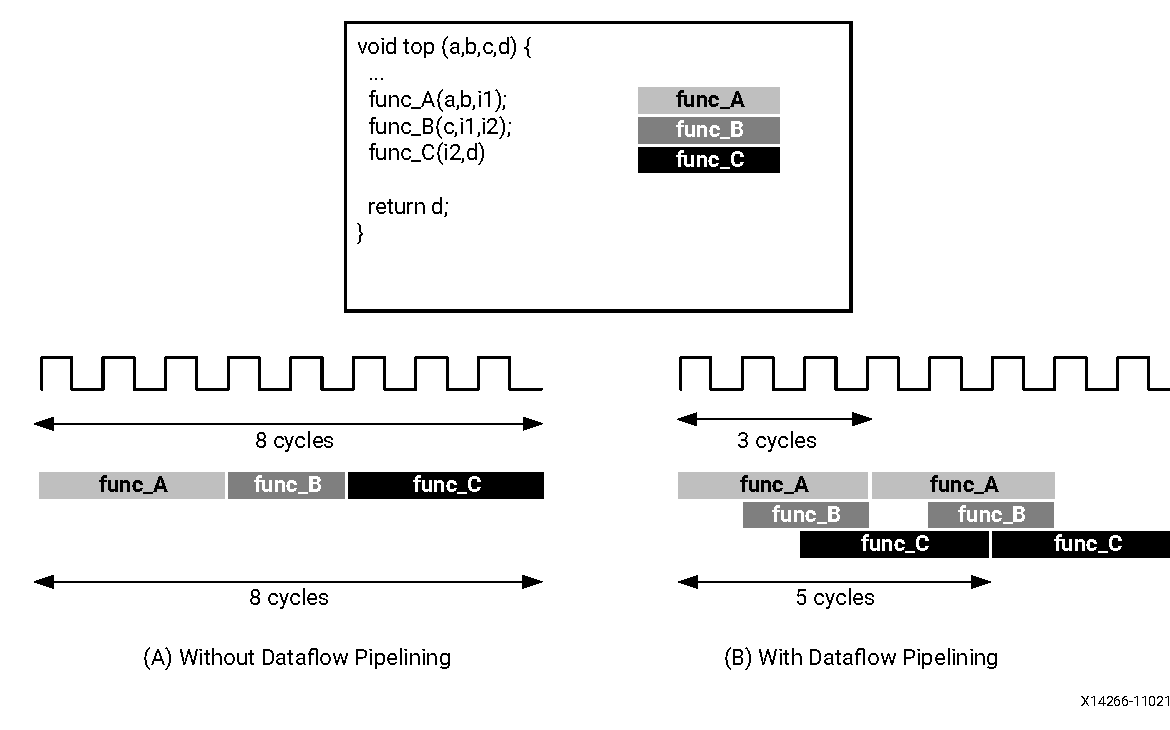
\includegraphics[width=0.82\textwidth]{Images/ug1399_dataflow.png}
    \caption[Task-level dataflow timing example]{Task-level dataflow timing example \cite{amd2026vitisHls}}
    \label{fig:ug1399_dataflow}
\end{figure}

In the proposed design, \texttt{DATAFLOW} is suitable for overlapping coarse-grained ResBlock stages. For example, Pass A performs convolution and writes intermediate output feature maps, while Pass B performs normalization, activation, and residual addition. When these stages are connected through FIFO or ping-pong buffers, the second stage can consume data while the first stage continues producing later rows or tiles. At the circuit level, \texttt{DATAFLOW} creates concurrently active processes connected by channels. At the timing level, it reduces idle cycles between stages and improves end-to-end throughput, provided that the producer and consumer rates are balanced.

\subsubsection{Summary of HLS Pragma Selection}

Table~\ref{tab:hls_pragmas_summary} summarizes the role of each pragma in the proposed generator accelerator. The key observation is that pragmas must be selected together. A pipelined MAC loop cannot reach \texttt{II=1} if the memory has insufficient ports. An unrolled PE cluster cannot be useful if the interface cannot supply data. Dataflow overlap is effective only when buffers decouple producer and consumer stages.

\begin{table}[H]
\centering
\caption{Summary of HLS pragmas used in the proposed generator accelerator}
\label{tab:hls_pragmas_summary}
\begin{tabularx}{\textwidth}{|p{0.22\textwidth}|X|X|X|}
\hline
\textbf{Pragma} & \textbf{Circuit effect} & \textbf{Timing effect} & \textbf{Suitable use in this thesis} \\
\hline
\texttt{PIPELINE II=1} & Adds pipeline scheduling and registers to loop/function datapaths & Starts a new iteration every cycle when dependencies allow & Inner MAC loops in each PE \\
\hline
\texttt{UNROLL factor=N} & Creates multiple copies of loop hardware & Reduces latency and increases parallel work per cycle & PE loops and SIMD channel lanes \\
\hline
\texttt{ARRAY\_PARTITION} & Splits arrays into memory banks or registers & Removes memory port conflicts and supports \texttt{II=1} & IFM buffers, weight buffers, and OFM arrays \\
\hline
\texttt{BIND\_OP} & Maps arithmetic to selected resources such as DSP or fabric & Controls operator latency and helps timing closure & FP16 multiplication inside PEs \\
\hline
\texttt{INTERFACE} & Generates AXI/control ports for top-level arguments & Enables efficient PS--PL and DDR communication & ResBlock top-level kernel connection \\
\hline
\texttt{DATAFLOW} & Creates concurrent tasks connected by FIFO/PIPO channels & Overlaps stages and reduces idle cycles & Convolution pass and normalization/activation pass \\
\hline
\end{tabularx}
\end{table}

Overall, HLS is appropriate for this thesis because the target workload is algorithmically complex but structurally regular. The designer can express the HiFiC ResBlock in C/C++, verify functionality at a high level, and use pragmas to control parallelism, memory bandwidth, arithmetic binding, interfaces, and task overlap. This approach provides a practical compromise between software-level productivity and hardware-level performance.


\subsection{Software Tools for Verification and Synthesis}

When designing FPGA-based accelerators for CNN workloads, verification and synthesis tools are essential for ensuring functional correctness, resource efficiency, and timing feasibility. The tool flow must support both algorithm-level validation and hardware-level implementation. In this thesis, the main software tools are Vivado for FPGA synthesis and system integration, Vitis for embedded software development, and PetaLinux for preparing the Linux-based runtime environment on the Zynq Processing System.

\subsubsection{Vivado}

Vivado is the FPGA design suite developed by Xilinx, now part of AMD, for synthesis, implementation, timing analysis, IP integration, and bitstream generation targeting Xilinx FPGA devices. After the HLS kernel has been verified and exported as an RTL IP core, Vivado is used to integrate the accelerator into the complete FPGA system.

In the proposed design flow, Vivado maps the generated RTL into FPGA resources such as LUTs, flip-flops, BRAMs, URAMs, and DSP slices. The synthesis stage converts the RTL description into a gate-level netlist, while the implementation stage performs placement and routing on the target device. Timing analysis is then used to check whether the design satisfies the required clock constraints. These steps are necessary for evaluating whether the generator accelerator can meet the target frequency and resource budget on the selected FPGA platform.

Vivado also provides IP Integrator and reusable IP cores for building a complete Zynq-based system. The accelerator IP can be connected to the Processing System, DDR memory controller, AXI interconnects, reset logic, and clocking blocks through a block design. After verification and implementation, Vivado generates the bitstream used to configure the Programmable Logic. In this thesis, Vivado therefore acts as the bridge between the HLS-generated accelerator and the deployable FPGA system.

\subsubsection{Vitis}

Vitis is AMD's unified software development platform for building, debugging, and deploying applications on heterogeneous Xilinx devices. In a Zynq-based system, Vitis is used after the hardware platform has been created in Vivado. The exported hardware description provides information about the Processing System, Programmable Logic, memory map, AXI interfaces, interrupts, and available hardware IP cores. Based on this platform, Vitis can generate the board support package and compile software that runs on the ARM processors in the PS.

For the proposed HiFiC GAN accelerator, Vitis is used to develop the host application that controls the hardware kernel. The software configures accelerator registers through AXI4-Lite, writes base addresses and tensor parameters, starts the accelerator, waits for completion, and reads back status or performance counters. It can also be used to measure end-to-end execution time and compare hardware acceleration against software execution. Therefore, Vitis connects the generated hardware accelerator with the software layer that manages data movement and execution control.

Vitis is also useful for debugging embedded applications because it supports compilation, launching, and step-by-step inspection on the target board or emulator. In this design flow, Vitis complements Vitis HLS: Vitis HLS focuses on generating the accelerator IP from C/C++ code, while Vitis focuses on writing and validating the PS-side application that uses that IP in the complete embedded system.

\subsubsection{PetaLinux}

PetaLinux is an AMD/Xilinx embedded Linux development environment for creating, configuring, building, and booting Linux images for FPGA SoC platforms. It provides command-line tools and build recipes that package the hardware description, bootloader, device tree, Linux kernel, root file system, and user applications into a deployable embedded Linux system. For Zynq UltraScale+ platforms, PetaLinux is especially useful because the PS can run Linux while the PL implements custom accelerator IP.

Fig.~\ref{fig:petalinux_flow} shows a typical PetaLinux development flow. The process starts from the hardware platform exported by Vivado. The designer then creates or selects a PetaLinux project using \texttt{petalinux-create}. Next, \texttt{petalinux-config} is used to import the hardware description and configure kernel options, root file-system packages, user applications, device-tree settings, and system parameters. After configuration, \texttt{petalinux-build} compiles the boot components, Linux kernel, device tree, and root file system. The optional \texttt{petalinux-package} step can package boot artifacts such as the boot image. Finally, \texttt{petalinux-boot} or an SD-card boot flow is used to run the generated Linux image on QEMU or on the target board.

\begin{figure}[H]
    \centering
    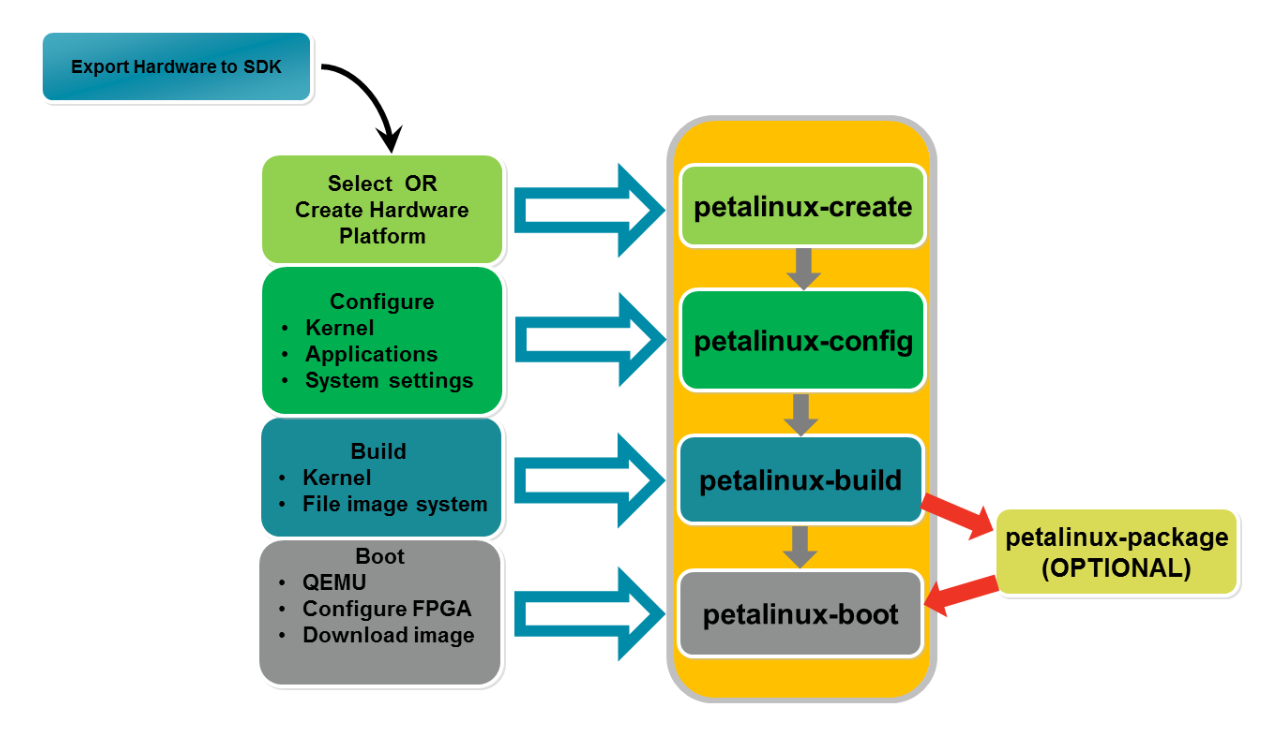
\includegraphics[width=0.9\textwidth]{Images/petalinux_flow.png}
    \caption{PetaLinux project creation, configuration, build, package, and boot flow}
    \label{fig:petalinux_flow}
\end{figure}

In the proposed system, PetaLinux provides the runtime environment for controlling the accelerator from software. The generated Linux image can include the required drivers, device-tree entries, libraries, and application files needed to access the accelerator IP and DDR memory from user space or kernel space. This makes PetaLinux the final deployment layer after the accelerator has been generated by Vitis HLS, integrated in Vivado, and controlled by software developed in Vitis.

\subsection{Chapter Conclusion}

Chapter 2 presented the theoretical background required for designing the proposed quantized HiFiC GAN accelerator. It first reviewed the main CNN operations used in learned image compression, including convolution, activation, normalization, residual connections, and up-sampling, and then introduced GANs and the HiFiC architecture together with the mixed-precision quantization concept used in this thesis. It also presented the evaluation metrics for both hardware efficiency and image-compression quality. These concepts explain the computational and memory-access characteristics that must be considered when mapping the ResBlock workload onto FPGA hardware.

The chapter then introduced the FPGA platform and explained why FPGA resources such as LUTs, flip-flops, on-chip memories, DSP slices, and AXI interfaces are suitable for accelerating CNN-based image compression. It also discussed the HLS design methodology, including scheduling, binding, pipelining, loop unrolling, array partitioning, operation binding, interface generation, and task-level dataflow. Finally, the chapter summarized the software tools used in the development flow, including Vitis HLS for accelerator generation, Vivado for FPGA synthesis and system integration, Vitis for embedded software development, and PetaLinux for building the Linux-based deployment environment.

Based on this background, the following chapters describe how the proposed generator accelerator is designed, optimized, integrated, and evaluated on the target FPGA platform.
